\section{Our Implementation: \nanomaly}
\label{sec:impl-nanomaly}
We have implemented our interactive semantics for the pure subset of
\ocaml with a web-based visualization of the generated traces in a tool
called \nanomaly.
%
It takes as input an \ocaml program and a function to check, searches
for a witness as described in \S~\ref{sec:searching-witness}, and
produces as output an interactive trace of the (possibly buggy)
execution~\footnote{If no witness could be found we simply return a trace
  of the last attempt.}.
%
We initially display a big-step reduction, \ie the source term followed
by the stuck term (or the final value).
%
The user can then progressively fill in the hidden steps of the
computation by selecting a visible term and choosing one of the
applicable traversal strategies -- described in
\S~\ref{sec:traversing-graph} -- to insert another term into the
visualization.

A sample interaction of the student program in
Figure~\ref{fig:palindrome} can be seen in
Figure~\ref{fig:nanomaly-palindrome}.
%
The initial state of the visualization tells us that the witness is
@palindrome []@, and that after some number of steps -- the thick arrow
denotes a multi-step transition -- we try to compare a function to a
list, which is not allowed in \ocaml.
%
Based on our semantics for \lang one would expect the final state to be
the \stuck term, but in practice we simply halt execution at the point
where an expression would transition to \stuck, as this final state is
more informative.
%
Note also that the equality test is colored black while the contextual
if-expression is faded out, this tells the user that the program got
stuck while trying to evaluate the sub-expression.

Upon seeing the stuck term, one might wonder where the @function@
came from.
%
To investigate we select the stuck term and click the ``jump backward''
button to search backwards from the stuck term for the most recent
function call, which brings us to @listReverse [] = w@, in the same
context as before.
%
Uncontent with the explanation so far, we ``step forward'' twice from
the @listReverse []@ term, bringing us to @helper [] = w@.
%
At this point it is clear that the @helper@ function is not defined
correctly, we have supplied it with the single argument we expected and
yet it still returned a @function@.

The problem is that the @function@ keyword in \ocaml defines an
anonymous function that takes a single argument and immediately does a
case-analysis without giving the argument a name.
%
The solution is to replace @function@ with an explicit @match xs with@
-- naming the value we wish to case-analyse.
%
After applying our fix, \nanomaly -- and more importantly \ocaml --
decide that @listReverse@ is safe to run.
\ES{these last few paragraphs probably belong in the overview}
%
\begin{figure}[t]
\centering
\begin{code}
  let listReverse l =
    let rec helper xs = function
      | [] -> xs
      | hd::tl -> helper (hd :: xs) tl
    in helper []

  let palindrome w =
    if listReverse w = w
    then true
    else false
\end{code}
\caption{Ill-typed \texttt{palindrome} function. The error lies in the
  use of the \texttt{function} construct which introduces an extra,
  undesired lambda abstraction, but manifests itself in the equality
  test on line XX. The fix is to replace \texttt{function} with
  \texttt{match xs with}. \ES{I think we should use this example in the
    intro/overview, leaving it here for now until they exist..}}
\label{fig:palindrome}
\end{figure}
%
\begin{figure}[t]
% \centering
Initial state: \\
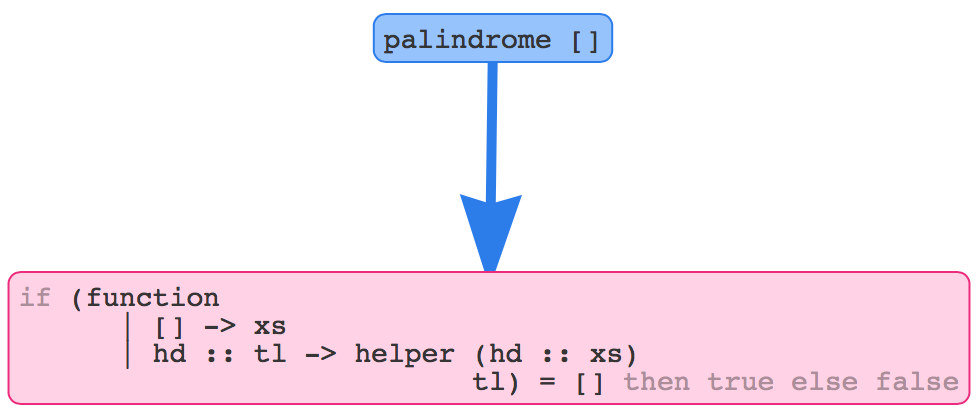
\includegraphics[width=\linewidth]{palindrome} \\
After ``jumping backward'' from the stuck term: \\
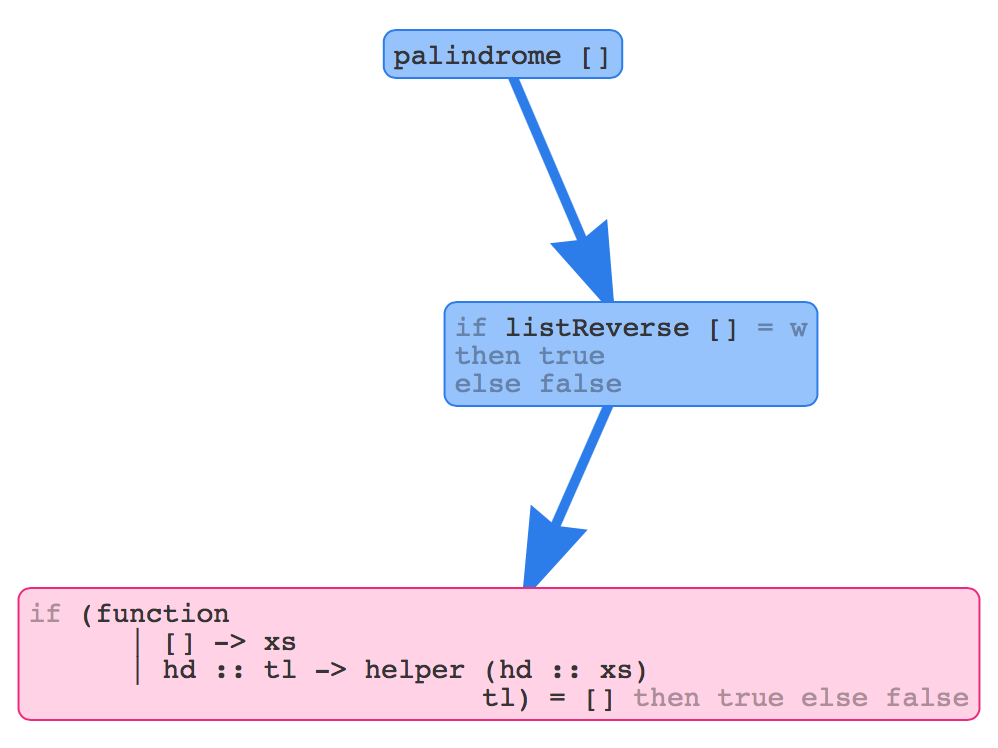
\includegraphics[width=\linewidth]{palindrome2} \\
After ``stepping forward'' twice from @listReverse []@: \\
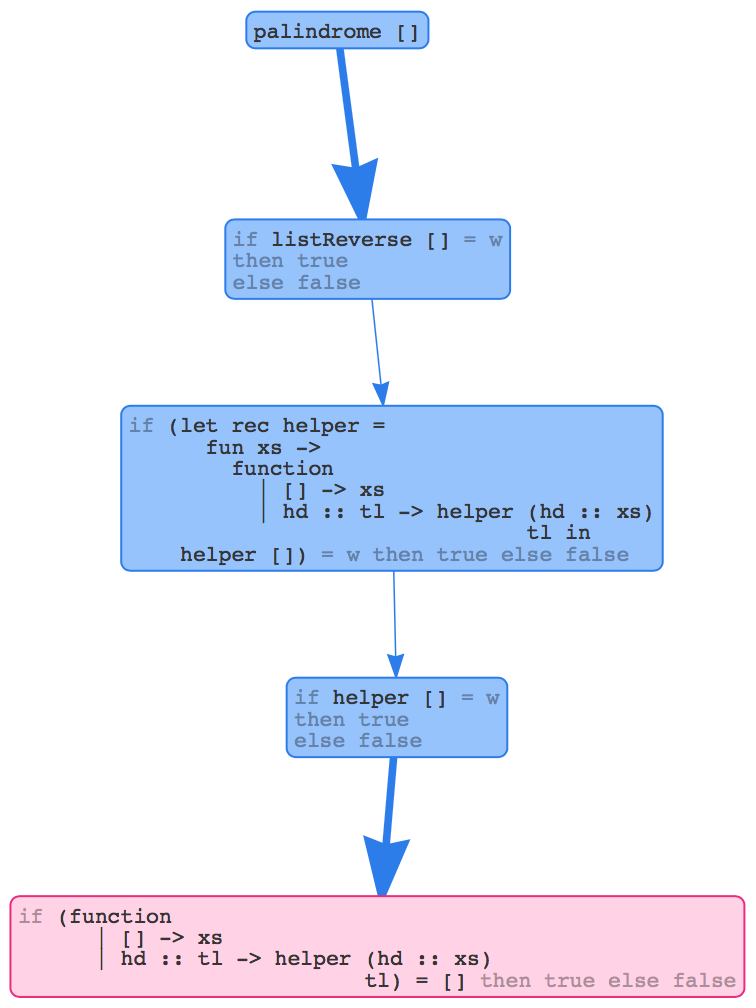
\includegraphics[width=\linewidth]{palindrome3} \\
\caption{Sample interaction}
\label{fig:nanomaly-palindrome}
\end{figure}

% !TEX root = main.tex
